\chapter{Analyse mit CryptoMiniSat}
\label{chp:analyse}

Die im letzten Kapitel erstellte konjunktive Normalform wird in diesem Kapitel für eine Analyse mit CryptoMiniSat verwendet.
Analyse bedeutet in diesem Fall, Lösungsversuche mit CryptoMiniSat durchzuführen. CryptoMiniSat sammelt dabei zusätzliches Wissen
in Form von Konfliktklauseln. Außerdem können durch die Optimierung der ursprünglichen konjunktiven Normalform weitere Klauseln
generiert werden. Sowohl die Konfliktklauseln als auch die aus der Optimierung entstandenen Klauseln sollen in diesem Kapitel
analysiert werden um die Module aus dem vorhergehenden Kapitel mit weiterem Wissen anzureichern und weitere Lösungsversuche zu
beschleunigen. Das Vorgehen ist dabei iterativ. Nach einem Lösungsversuch werden mutmaßlich wertvolle Klauseln identifiziert
und in die Module aufgenommen, um mit diesem zusätzlichen Wissen einen weiteren Lösungsversuch zu starten.

Als Lösungsversuch wird die Urbildberechnung (siehe Abschnitt \ref{sec:urbildberechnung}) herangezogen. Die Initialwertberechnung
(siehe Abschnitt \ref{sec:initialwertberechnung}) eignet sich nicht, da die Eingabe bekannt ist und somit die Erweiterung der Eingabe
vollständig berechnet werden kann. Dadurch ist dieser Teil bereits gelöst und wird im Lösungsversuch nicht berücksichtigt. Das führt
dazu, dass kein Wissen über die Erweiterung der Eingabe erworben werden kann. Für die Urbildberechnung wird der \glos{hash} aus Abbildung
\ref{fig:ruby-sha256} herangezogen. Dieser wurde aus der Eingabe "`Das ist eine Eingabe aus der ein \glos{hash} erstellt wird."' mit Hilfe
der interaktiven Rubykonsole berechnet und dient unter anderem auch als Testfall für die Kompressionsfunktion. Ziel des Lösungsversuchs
ist es, eine Eingabe mit 52 Byte Länge zu finden. Dies könnte auch die Eingabe sein, die benutzt wurde um den \glos{hash} zu berechnen.
\begin{figure}[!h]
  \centering
  \begin{lstlisting}[]
  require 'digest'
  Digest::SHA256.hexdigest 'Das ist eine Eingabe aus der ein Hash erstellt wird.'
                        => "27931f0e7e53670ddbec1a1ce23e21b4663c63c0d17117ee1a934bc0c294dbe9"
  \end{lstlisting}
  \caption{Ruby - \glos{sha256}}
  \label{fig:ruby-sha256}
\end{figure}

Beachtet werden muss auch, dass der \glos{hash} nicht direkt mit in die konjunktive Normalform kodiert wird. Gleiches gilt für die \glospl{initialwert}
und das Padding, was vorgegeben wird um die Eingabelänge zu definieren. Eine direkt Kodierung würde dazu führen, dass erworbenes Wissen
sich auf diese Werte bezieht und somit nur für diesen Fall gültig ist. Um das zu vermeiden werden alle Werte als "`Annahmen"' (Assumptions)
an CryptoMiniSat übergeben. Das führt dazu, dass die Werte zwar für diesen Lösungsversuch gelten, jedoch nicht als allgemeingültig betrachtet
werden. Klauseln die auf diesem Wissen basieren, werden separat behandelt und nach dem Lösungsversuch verworfen (in Anlehnung an
"`Incremental Satisfiability"' \cite[Kapitel 6]{shtrichman}).

Ebenfalls berücksichtigt werden muss die Extraktion der gelernten Klauseln aus CryptoMiniSat. Die internen Datenstrukturen sind nicht dafür
geeignet, die Klauseln während eines laufenden Lösungsversuchs zu extrahieren. Eine Extraktion kann nur erfolgen, wenn CryptoMiniSat eine
Lösung gefunden hat wobei die Lösung auch sein kann, dass es keine Lösung gibt. Wie zu erwarten ist, kommt CryptoMiniSat aber bei vollständiger
Vorgabe des \glos{hash} zeitnah zu keiner Lösung. Deshalb wird ein iterativer Ansatz verfolgt. Die \glospl{initialwert} und das Padding werden immer vollständig vorgeben,
während die Vorgabe des \glos{hash} bitweise erweitert wird. Nach jeder Lösung werden dabei die Klauseln extrahiert. Es werden so lange Bits des \glos{hash}
ergänzt, bis keine Lösung mehr gefunden wird. Im Allgemeinen zeigt sich dies dadurch, dass CryptoMiniSat aufgrund eines vollen Hauptspeichers
abstürzt oder das Programm selbst die Menge der Klauseln nicht mehr handhaben kann.

Extrahiert werden in jedem Lösungsversuch die irredundanten und die redundanten Klauseln. Die irredundanten Klauseln enthalten zunächst die
eingegebene konjunktive Normalform, die jedoch während der Lösungsversuche optimiert wird. Die redundanten Klauseln enthalten das gelernte
Wissen, das zusätzlich genutzt wird und wegfallen könnte, ohne die Lösungsmenge zu beeinflussen.

In den folgenden Abschnitten wird die Analyse der extrahierten Klauseln im Detail beschrieben. Zunächst werden in Abschnitt \ref{sec:ana:rem_double}
alle Klauseln gesammelt und schon bekannte Klauseln aussortiert. In Abschnitt \ref{sec:ana:module} wird versucht, die Klauseln einzelnen Modulen
zuzuordnen und diese zu normalisieren. Gelingt die Zuordnung zu einem Modul nicht, wird in Abschnitt \ref{sec:ana:distance} eine Distanzmetrik
genutzt, um die Klauseln zu bewerten und mutmaßlich wertvolle Klauseln zu identifizieren. Die Verallgemeinerung von Klauseln über die Breite von
32 Bit und die 64 Runden von \glos{sha256} wird in Abschnitt \ref{sec:ana:generalize} betrachtet. Durch die Iterationen, die jeweils gelerntes Wissen mit
einbeziehen, kann es dazu kommen, dass Dont-Care Literale identifiziert werden und zur Verkürzung von Klauseln führen. Diese Entwicklung wird in
Abschnitt \ref{sec:ana:subclauses} betrachtet. Abschließend wird das gelernte Wissen in Abschnitt \ref{sec:ana:acquired} zusammengefasst.

\section{Aussortieren bekannter und doppelter Klauseln}
\label{sec:ana:rem_double}

Da die Entscheidung, ob eine XOR-Unterstützung vorliegt, beim Kompilieren getroffen werden muss, werden die bekannten Klauseln
mit dem Programm "`dimacsprinter"' nach jedem Lösungsversuch und der darauf folgenden Analyse in zwei Dateien im DIMACS-Format
ausgegeben. Die eine Datei enthält dabei die Klauselmenge ohne XOR-Unterstützung während die andere Datei die Klauselmenge für
eine XOR-Unterstützung enthält. Das Programm "`clausecollector"' liest beide Dateien beim Start ein und führt die Klauselmengen
zusammen. Da CryptoMiniSat XOR-Klauseln akzeptiert, diese jedoch intern in normale Klauseln umrechnet, enthalten auch die
extrahierten Klauseln keine XOR-Klauseln. Der Parser für das DIMACS-Format konvertiert deshalb ebenfalls XOR-Klauseln in normale
Klauseln.

Abgelegt werden die bekannten Klauseln in einem "`set"'. Diese Datenstruktur ermöglicht die Suche nach einer Klausel in logarithmischer
Zeit im Bezug zur Anzahl der darin enthaltenen Klauseln. So kann effizient geprüft werden, ob eine extrahierte Klausel schon bekannt ist.
Neue Klauseln aus der irredundanten und der redundanten Klauselmenge werden ebenfalls jeweils in einem "`set"' gesammelt wodurch die
Klauselmenge automatisch sortiert wird und doppelte Klauseln wegfallen. Abschließend werden die neuen Klauseln aus der irredundanten und
der redundanten Klauselmenge jeweils in in eine DIMACS-Datei zur weiteren Analyse geschrieben.
\section{Erkennen und normalisieren modulspezifischer Klauseln}
\label{sec:ana:module}

Nach dem Aussortieren der schon bekannten Klauseln werden die neuen Klauseln den einzelnen Modulen zugeordnet. Durch die hierarchische Anordnung
muss beachtet werden, dass eine Klausel mehreren Modulen zugeordnet werden kann. Sinnvoll ist es jedoch, die Klausel nur dem Modul zuzuordnen,
das in der Hierarchie möglichst weit unten steht. Wird eine Klausel für einen Addierer gefunden, kann diese Klausel so zukünftig für alle Addierer
genutzt werden, während sie im Modul für die vollständige Kompressionsfunktion nur für den einen speziellen Addierer gelten würde. Um diese
Zuordnung zu realisieren, erhält jedes Modul ein Level. Im hierarchischen Aufbau muss das Level eines Moduls dabei höher sein als das höchste Level
der verwendeten Module. Die vergebenen Level sind in Abbildung \ref{fig:sha256_module_level} dargestellt.
\begin{figure}[!h]
  \centering
  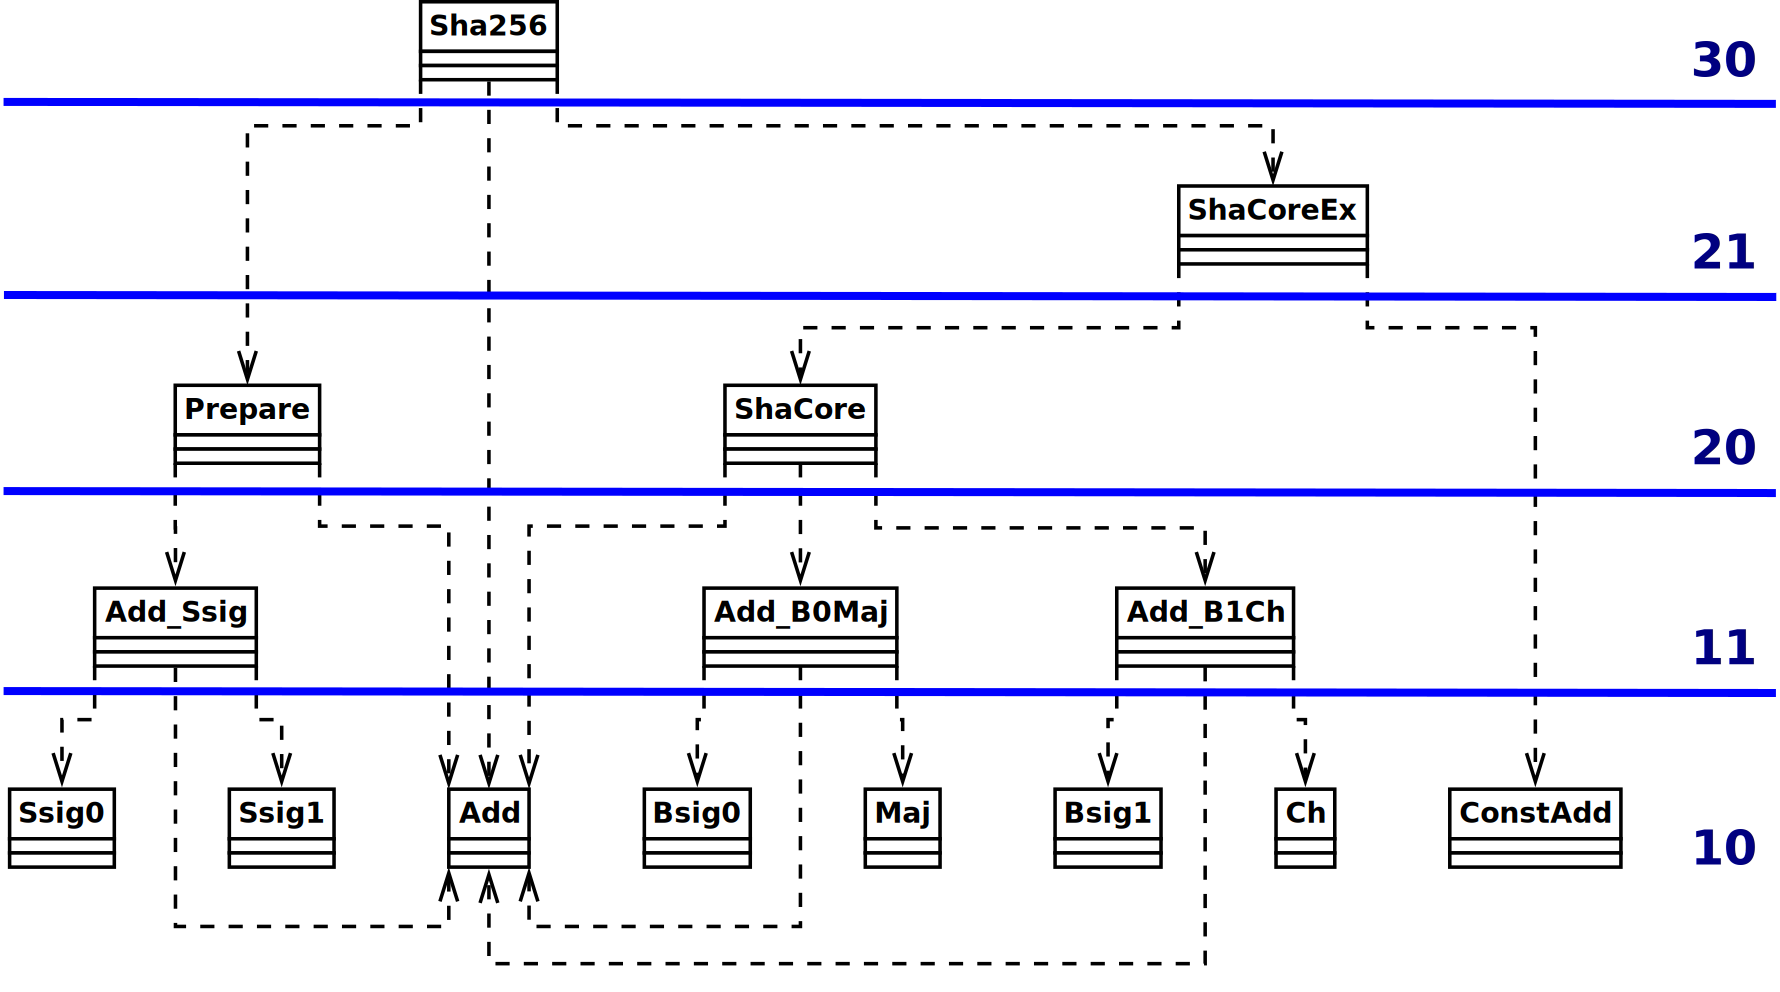
\includegraphics[scale=0.265]{images/module_level}
  \caption{Modullevel von \glos{sha256}}
  \label{fig:sha256_module_level}
\end{figure}

Die Level werden nicht fortlaufend nummeriert, um bei Bedarf weitere Module/Level einfügen zu können, ohne die Level der vorhandenen Module anpassen zu müssen.

Anhand der Level können die Module sortiert werden, so dass die Prüfung, ob eine Klausel zum Modul gehört, bei den Modulen mit dem niedrigsten Level beginnen kann.
Eine Klausel gehört dann zu einem Modul, wenn alle Literale der Klausel im Modul verwendet werden. Dabei kann es sich um Eingänge, zusätzliche Literale oder Ausgänge
handeln. Ein Sonderfall ist eine Klausel, die ausschließlich aus Eingangsliteralen oder ausschließlich aus Ausgangsliteralen besteht. Die Ausgangsliterale eines Moduls
sind im Allgemeinen die Eingangsliterale eines anderen Moduls, wodurch die Zuordnung bei gleichem Level unklar ist. Klauseln dieser Art wurden bei der Analyse jedoch
nicht gefunden. 

Für die Zuordnung der Klauseln wird zunächst ein Collector mit dem Namen "`ModulDB"' implementiert. Die ModulDB überschreibt nur die Methode newModul des Collectors,
um die Registrierung der Module zu erfassen. Generierte Klauseln, die an die Methode create übergeben werden, werden dadurch ignoriert. Erfasst werden neben dem
Modulnamen und dem Level die verwendeten Literale in der Reihenfolge: Eingänge, zusätzliche Literale und Ausgänge. ModulDB stellt außerdem eine Funktion bereit,
der eine beliebige Klausel zur Zuordnung übergeben werden kann. Wird ein passendes Modul gefunden, wird ein Zeiger auf die Modulinformationen zurückgeliefert.

Das Programm "`modulchecker"' nutzt schließlich die ModulDB für die Zuordnung. Zunächst wird ein Objekt der Kompressionsfunktion erzeugt, in das die ModulDB als
Besucher übergeben wird. Danach werden die im vorigen Abschnitt erstellten DIMACS-Dateien eingelesen und jede Klausel einem Modul zugeordnet. Die Zuordnung wird
in diesem Fall immer gelingen, weil spätestens die Kompressionsfunktion alle Literale umfasst.

Da die Module in ihrer Normalform implementiert werden (siehe Kapitel \ref{chp:knf}), kann eine zugeordnete Klausel noch nicht direkt genutzt werden.
Die verwendeten Literale in der Kompressionsfunktion sind andere als die des Moduls in der Normalform. Wird eine Klausel zugeordnet, erfolgt deshalb
direkt im Anschluss die Normalisierung der Klausel. Diese wird auf Basis der im Modul verwendeten Literale durchgeführt. Da diese in der richtigen
Reihenfolge vorliegen, können in der Klausel vorkommende Literale darin erkannt und anhand des Index in das Literal der Normalform überführt werden.

Nach der Normalisierung werden die Klauseln für jedes Modul in einem eigenen "`set"' gesammelt. Wie in Abschnitt \ref{sec:ana:rem_double} erfolgt
dadurch eine automatische Aussortierung doppelter Klauseln. Diese ist erneut notwendig, weil Module mehrfach an verschiedenen Stellen verwendet werden.
Klauseln, die vorher unterschiedlich sind, werden durch die Normalisierung zu gleichen Klauseln, wenn das gleiche Wissen über ein Modul an mehreren
Stellen erworben wurde.

Abschließend werden die neuen Klauseln jedes Moduls in eine eigene DIMACS-Datei geschrieben. Bevor diese Klauseln in die Module integriert werden können, ist
es notwendig die Gültigkeit zu überprüfen. Ungültig kann eine Klausel dann sein, wenn sie sich aus dem Kontext, in dem das Modul verwendet wurde, ergibt.
In diesem Fall ist es notwendig, die Klausel auf ein Modul höheren Levels zu übertragen. Die Gültigkeitsprüfung wird mit dem Programm "`clausechecker"'
durchgeführt. Dabei werden die bekannten Klauseln des Moduls an CryptoMiniSat übergeben. Jede (neue) Klausel lässt sich als nicht erfüllbare Belegung
interpretieren und wird deshalb als Annahme bei einem Lösungsversuch übergeben. Gelingt es CryptoMiniSat nicht, eine Lösung zu finden, ist die Gültigkeit
der Klausel bestätigt. In dieser Arbeit haben sich jedoch alle überprüften Klauseln als gültig herausgestellt und brauchen nicht auf ein Modul höheren
Levels übertragen zu werden.

Nur ein kleiner Teil (< 5\%) der neuen Klauseln lässt sich einem Modul unterhalb des Levels 30 zuordnen. Der Großteil ergibt sich aus dem Zusammenspiel
der Erweiterung der Eingabe und der Rundenfunktion und wird somit dem Modul für die Kompressionsfunktion zugeordnet. Der Versuch alle diese Klauseln
in einen weiteren Lösungsversuch einzubringen hat gezeigt, dass dadurch der Lösungsprozess deutlich verlangsamt wird. Daraus ergibt sich die Notwendigkeit,
diese Klauseln einer weiteren Analyse zu unterziehen, die im folgenden Abschnitt erläutert wird.
\section{Distanzermittlung von Klauseln außerhalb der Module}

\TODO{erledigen}
\section{Verallgemeinerung von Klauseln}
\label{sec:ana:generalize}

Bisher erhaltene Klauseln werden in diesem Abschnitt darauf untersucht, ob eine Verallgemeinerung möglich ist. Verallgemeinerung bedeutet dabei, den Sinn der Klausel
zu erkennen und auf weitere Stellen anzuwenden. Auf Modulebene erfolgt dieser Prozess bereits automatisch, da diese Klauseln überall dort angewendet werden, wo das
Modul zum Einsatz kommt. Eine weitere Möglichkeit ist es, weitere Stellen innerhalb des Moduls zu identifizieren, an denen die Klausel ebenfalls gültig ist. Besonders
gut funktioniert diese Verallgemeinerung bei dem Addierer. Durch die Breite von 32 Bit können viele Klauseln bitweise nach vorne oder hinten verschoben werden und sind
an diesen Stellen ebenfalls gültig. Aufgrund der Vielzahl der erhaltenen Klauseln ist jedoch eine weitere Unterteilung notwendig. Zunächst werden die in Abschnitt
\ref{sec:knf:addierer} erläuterten Komponenten des Addierers (Halb-, Voll- und Mod-2 Addierer) in eigene Module mit dem Level eins ausgelagert. Dadurch können viele
Klauseln direkt den Halb-, Voll und Mod-2 Addiereren zugeordnet werden. Ein Großteil der erworbenen Klauseln verbleibt aber nach wie vor im Modul des 32-Bit Addierers.
Bei der Analyse der verbleibenden Klauseln zeigt sich, dass sich diese Klauseln in Halb-, Voll und Mod-X Addiereren höherer Ebene organisieren lassen. Als Addierer
höherer Ebene wird ein Addierer bezeichnet, der bei Bedarf ein eingehendes oder ausgehendes Carrybit berücksichtigt, intern jedoch keine Carrybits verwendet. Diese
Addierer entsprechen dem Carry-Lookahead Addierer (siehe Abschnitt \ref{sec:grundlagen_add}) in unterschiedlichen Bitbreiten. Ergänzt werden Module für Addierer bis
vier Bit Breite. Abbildung \ref{fig:sha256_module_add} zeigt die Erweiterung der Modulhierarchie.
\begin{figure}[!h]
  \centering
  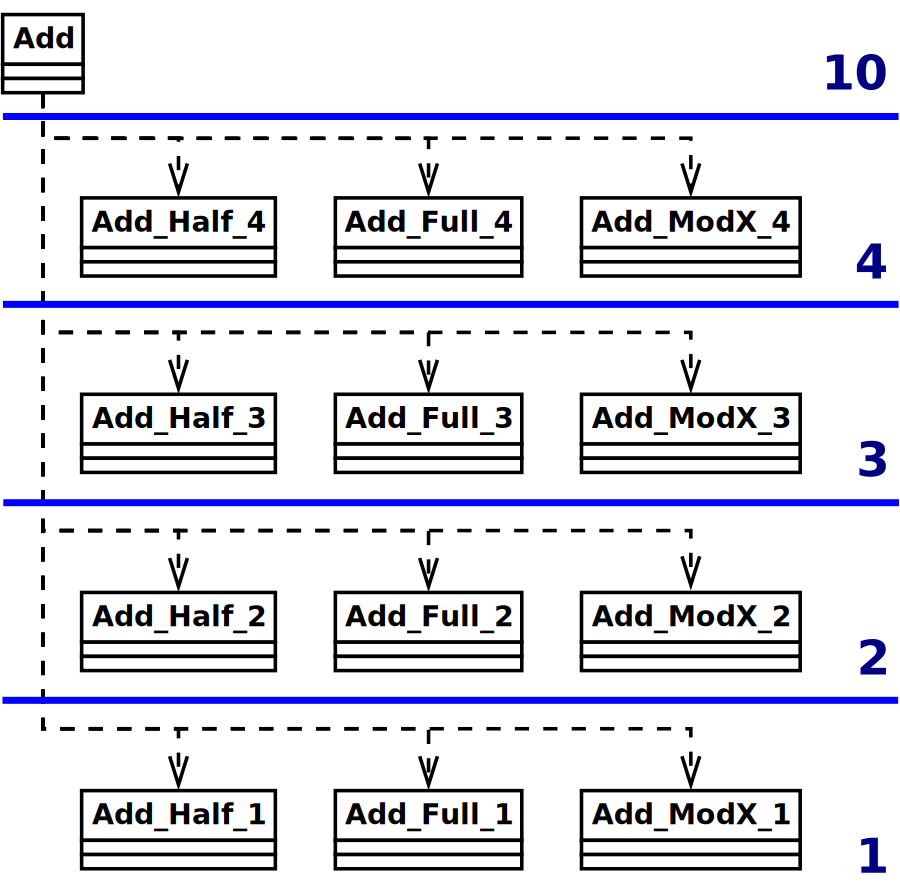
\includegraphics[scale=0.265]{images/module_add}
  \caption{Ergänzte Module von \glos{sha256}}
  \label{fig:sha256_module_add}
\end{figure}

Module für Addierer mit mehr als vier Bit Breite werden nicht ergänzt, da der SAT-Solver keine Klauseln ermittelt hat, die diesen Modulen zugeordnet werden konnten.  
Notwendig für die Funktion des Addierers sind nur die Module mit dem Level eins. Die Module mit dem Level zwei bis vier dienen als zusätzliche Information
auf den selben Literalen. Durch dieses Vorgehen erfolgt die Verallgemeinerung von Klauseln innerhalb des Addierers ebenfalls automatisch.

Bei den anderen Modulen zeigt sich kein Muster dieser Art und die Anzahl der erworbenen Klauseln ist vergleichsweise gering. Deshalb werden die erworbene Klauseln
darin direkt untergebracht und durch Verwendung einer Schleife verallgemeinert in sofern dies möglich ist. Eine Ausnahme bildet das Modul der vollständigen
Kompressionsfunktion. Neben der Verallgemeinerung auf Bitbreite bietet sich in diesem Modul die Möglichkeit, die Klauseln auch auf weitere Runden anzuwenden.
Klauseln die sich nur auf eine Runde beziehen wurden schon dem Modul für die Rundenfunktion zugeordnet, so dass nur noch Klauseln betrachtet werden die sich über
zwei oder mehr Runden erstrecken. Jedes Literal der jeweiligen Klausel wird um eine Runde nach vorne oder hinten verschoben.

Beachtet werden muss, dass jede der 64 Runden eine andere Rundenkonstante verwendet und die Erweiterung der Eingabe bei den ersten 16 Runden keine
Anwendung findet. Während bei den anderen Modulen im Allgemeinen eine Verallgemeinerung entweder funktioniert oder nicht, muss dadurch jede durch die
Verallgemeinerung generierte Klausel einzeln überprüft werden. Wie auch bei der Überprüfung der modulspezifischen Klauseln in Abschnitt \ref{sec:ana:module}
wird das Programm "`clausechecker"' für die Überprüfung genutzt. Nur wenige der ermittelten Klauseln lassen sich ohne Einschränkungen auf weitere Bits oder
Runden übertragen. Der clausechecker generiert deshalb ein zweidimensionales Array, in dem die gültigen Klauseln markiert werden. Dieses Array wird im
Modul der Kompressionsfunktion genutzt, um die gültigen Klauseln in die konjunktive Normalform zu integrieren. Es zeigt sich, dass die Werte des Arrays in
einigen Fällen die Rundenkonstante widerspiegeln. Im diesem Fall wird auf das Array verzichtet und die Bits der Rundenkonstante verwendet.

Es stellt sich heraus, dass dieses Vorgehen sehr erfolgreich ist weitere gültige Klauseln zu generieren. Auch Klauseln mit einer großen Distanz in der Kompressionsfunktion
lassen sich oft auf 400 bis 700 weitere Stellen übertragen, wobei CryptoMiniSat davon nur wenige gefunden hat. In der iterativen Anwendung zeigt sich, dass die
generierten Klauseln im nächsten Durchlauf dabei helfen, weitere Klauseln mit positiver Distanz zu finden.
\section{Subklauselprüfung}
\label{sec:ana:subclauses}

Durch die mehrfache iterative Anwendung der Methodik aus den letzten Abschnitten, kommt es zu einer kontinuierlichen Erweiterung der Klauselmenge.
Dazu zählt auch, dass Don't-Care Literale in Klauseln identifiziert und entfernt werden. Wenn die neuen kürzeren Versionen dieser Klauseln durch die
Analyse in die Klauselmenge aufgenommen werden, sind die alten langen Klauseln überflüssig. Um diese zu erkennen, wird das Programm "`clausesorter"'
genutzt. Dieses bekommt als Eingabe alle bekannten Klauseln und überprüft diese auf kürzere Klauseln. Die naive Variante hat eine quadratische
Laufzeit im Bezug zur Eingabegröße, weil zu jeder Klausel alle weiteren überprüft werden müssen. Um die Laufzeit zu reduzieren, wird eine Lookup-Tabelle
genutzt, in der zu jedem Literal die Klauseln hinterlegt sind, die das Literal enthalten. So werden zu jeder Klausel nur noch die Klauseln überprüft,
die mindestens ein gemeinsames Literal haben. Dieses Vorgehen entspricht dem Watchlist-Prinzip, das auch im SAT-Solver "`zChaff"' \cite{zmmm} Verwendung
findet. In der Praxis reduziert sich die Laufzeit bei zwei Millionen Klausel dadurch von einer Woche auf fünf Minuten.

Die als überflüssig erkannten Klauseln werden in eine separate Datei ausgegeben und genau wie neue Klauseln einem Modul zugeordnet. Dadurch können
diese Klauseln in den Modulen erkannt und entfernt werden. Zu Dokumentationszwecken werden die Klauseln nur auskommentiert. Eine Ausnahme bildet
die Kompressionsfunktion, in der die Klauseln mit positiver Distanz enthalten sind. Der Aufwand, die überflüssige Klausel im Programmcode zu identifizieren,
ist bei geringem Nutzen vergleichsweise hoch. Das Modul, und somit jede enthaltene Klausel, wird nur einmal verwendet. Die Anzahl der überflüssigen
Klauseln ist damit am Ende verhältnismäßig gering und sollte CryptoMiniSat nicht bremsen.

\section{Erhaltene Klauseln}
\label{sec:ana:acquired}

Nach der mehrfachen iterativen Anwendung der Methodik aus den letzten Abschnitten, wird die Analyse beendet. Bei den letzten Iterationen konnten
keine weiteren Klauseln sinnvoller Länge für die Module gefunden werden. Anders ist die Situation bei Klauseln aus der Kompressionsfunktion mit
positiver Distanz. Nach wie vor werden Klauseln generiert, die bei gleicher Distanz tendenziell kürzer werden. Da aber bisher nicht bekannt ist,
ob diese Klauseln den Lösungsprozess tatsächlich beschleunigen, wird die Analyse beendet.

Tabelle \ref{fig:additional_clauses_add} zeigt zunächst die erhaltenen Klauseln für die zusätzlichen Komponenten des Addierers.
Die Halb- und Mod-X-Addierer sind jeweils einmal enthalten, während die Volladdierer mit zwei bis vier Bit 29 bis 27 Mal enthalten sind.
Dadurch ergeben sich für den Addierer selbst insgesamt die zusätzlichen Klauseln in der unteren Zeile.
\begin{table}[!h]
  \centering
  \begin{tabular}{l|R{1.5cm}R{1.5cm}R{1.5cm}R{1.5cm}R{1.5cm}}
    \hiderowcolors
          & \multicolumn{5}{c}{\textbf{Klausellänge}} \\
    \cline{2-6}
    \textbf{Modul} & \textbf{3} & \textbf{4} & \textbf{5} & \textbf{6} & \textbf{7} \\
    \hline
    \showrowcolors
    Add\_Half\_$2$ & 9 &  16 &    9 &     &    \\
    Add\_Full\_$2$ &   &  22 &   38 &     &    \\
    Add\_ModX\_$2$ &   &     &   24 &     &    \\
    Add\_Half\_$3$ &   &   4 &    9 &   6 &    \\
    Add\_Full\_$3$ &   &     &   17 &  33 &    \\
    Add\_ModX\_$3$ &   &     &      &  27 &    \\
    Add\_Half\_$4$ &   &     &    5 &   2 &  4 \\
    Add\_Full\_$4$ &   &     &      &     &    \\
    Add\_ModX\_$4$ &   &     &      &     & 16 \\
    \hline
    Add          & 9 & 658 & 1625 & 959 & 20 \\
  \end{tabular}
  \caption{Erworbene Klauseln im Addierer}
  \label{fig:additional_clauses_add}
\end{table}

Erkennen lässt sich, dass die Länge der Klauseln mit der Ebene der Komponenten zunehmen. Gleichzeitig nimmt die Anzahl der erhaltenen Klauseln ab.
Das lässt sich dadurch erklären, dass bspw. ein 3-Bit Volladdierer auf den Literalen arbeitet, auf denen bereits zwei 2-Bit Volladdierer und drei
Volladdierer vorhanden sind. Damit ist ein Großteil des Verhaltens bereits definiert und es werden nur zusätzliche Klauseln benötigt, die bisher
fehlendes Verhalten definieren.

Tabelle \ref{fig:additional_clauses_mod} zeigt, wie viele Klauseln mit welcher Anzahl Literale in den essentiellen Modulen gefunden werden konnten.
Dazu gehören sowohl normale Klauseln als auch XOR-Klauseln. Sind in einer Zelle zwei Werte aufgeführt, gibt der erste Wert die Anzahl der zusätzlichen
Klauseln bei einer XOR-Unterstützung an. Der zweite Werte gibt die Anzahl der zusätzlichen Klauseln ohne XOR-Unterstützung wieder.
\begin{table}[!h]
  \centering
  \begin{tabular}{l|R{1.5cm}R{1.5cm}R{1.5cm}R{1.5cm}R{1.5cm}R{1.5cm}}
    \hiderowcolors
          & \multicolumn{6}{c}{\textbf{Klausellänge}} \\
    \cline{2-7}
    \textbf{Modul} & \textbf{2} & \textbf{3} & \textbf{4} & \textbf{5} & \textbf{6} & \textbf{7} \\
    \hline
    \showrowcolors
    Add\_Half\_$1$       & 1 & 2 - 3 &         &          &     &    \\
    Add\_Full\_$1$       &   & 6 - 8 &   0 - 2 &          &     &    \\
    Add\_ModX\_$1$       &   &       &         &          &     &    \\
    Add                  &   &     9 &     658 &     1625 & 959 & 20 \\
    Ssig$0$ ($\sigma_0$) &   &       &         & 3 - ~~48 &     &    \\
    Ssig$1$ ($\sigma_1$) &   &       &         &  7 - 112 &     &    \\
    Bsig$0$ ($\Sigma_0$) &   &       &         &          &     &    \\
    Bsig$1$ ($\Sigma_1$) &   &       &         &          &     &    \\
    Choose               &   &    64 &         &          &     &    \\
    Majority             &   &       &         &          &     &    \\
    Add\_Ssig            &   &       &       8 &          &     &    \\
    Add\_B$0$Maj         &   &       &         &          &     &    \\
    Add\_B$1$Ch          &   &       &     244 &      122 &     &    \\
    Prepare              & 2 &     8 &      68 &          &     &    \\
    ShaCore              & 3 &    32 & 81 - 95 &        1 &     &    \\
  \end{tabular}
  \caption{Erworbene Klauseln in den Modulen}
  \label{fig:additional_clauses_mod}
\end{table}

Der Mod-2 Addierer verwendet, genau wie die $\Sigma$-Funktionen, ausschließlich den XOR-Operator. Weitere Klauseln waren darin deshalb nicht zu erwarten und
wurden auch nicht gefunden. Bei den $\sigma$-Funktionen konnten weitere Klauseln gefunden werden, weil bei diesen, im Gegensatz zu den $\Sigma$-Funktionen, der
Shift-Operator verwendet wird, durch den einige Bits verworfen werden. Das zeigt sich auch bei der Addition der Ergebnisse der $\sigma$-Funktionen, wo ebenfalls
einige Klauseln gefunden werden konnten.

Im Modul der Choose-Funktion wurden zwei weitere Klauseln gefunden, die sich auf die Breite von 32 Bit anwenden lassen. Dadurch ergeben sich
64 zusätzliche Klauseln. Im Gegensatz dazu konnten bei der Majority-Funktion keine weiteren Klauseln gefunden werden. Dieses Muster findet sich auch
in den Modulen wieder, in denen das Ergebnis der Choose- und Majority-Funktion mit den Ergebnissen der $\Sigma$-Funktionen addiert wird. Nur in dem
Modul, in dem die Choose-Funktion verwendet wird (Add\_B$1$Ch), konnten weitere Klauseln gefunden werden.

Erfolgreicher ist die Ausbeute bei der Erweiterung der Eingabe (Prepare) und der Rundenfunktion (ShaCore). In diesen Modulen konnten einige Klauseln gefunden
werden, die sich aus dem Zusammenspiel zwischen Modulen kleineren Levels ergeben.

In der Kompressionsfunktion wurden die Klauseln mit positiver Distanz aus Tabelle \ref{fig:additional_clauses} ermittelt.
Basis für die insgesamt 29703 Klauseln bildeten 1107 Klauseln aus CryptoMiniSat. 28596 Klauseln wurden durch die Verallgemeinerung
auf Bitbreite und Runden ermittelt.
\begin{table}[!h]
  \centering
  \begin{tabular}{r|R{1.5cm}R{1.5cm}R{1.5cm}R{1.5cm}R{1.5cm}|R{1.5cm}}
    \hiderowcolors
          & \multicolumn{5}{c}{\textbf{Klausellänge}} \\
    \cline{2-6}
    \textbf{Distanz} & \textbf{2} & \textbf{3} & \textbf{4} & \textbf{5} & \textbf{6} & $ \boldsymbol{\sum} $ \\
    \hline
    \showrowcolors
                        1 & 428 &  412 &       &      &      &   840 \\
                        2 &  50 & 5287 &       &      &      &  5337 \\
                        3 &     &  159 &  9560 & 1430 &      & 11149 \\
                        4 &     &  318 &  1829 & 2068 & 5787 & 10002 \\
                        5 &     &   28 &   188 & 1469 &  718 &  2403 \\
    \hline
    $ \boldsymbol{\sum} $ & 478 & 6204 & 11577 & 4967 & 6505 & 29731 \\
  \end{tabular}
  \caption{Erworbene Klauseln in der Kompressionsfunktion}
  \label{fig:additional_clauses}
\end{table}

Wie in Abschnitt \ref{sec:ana:subclauses} erwähnt sind von diesen Klauseln einige überflüssig, weil bereits Don't-Care Literale identifiziert wurden
und kürzere Klauseln vorhanden sind. Tabelle \ref{fig:additional_clauses_clean} zeigt die Anzahl der sinnvollen Klauseln. 8425 Klauseln haben sich
als überflüssig herausgestellt, womit 21306 sinnvolle Klauseln verbleiben.
\begin{table}[!h]
  \centering
  \begin{tabular}{r|R{1.5cm}R{1.5cm}R{1.5cm}R{1.5cm}R{1.5cm}|R{1.5cm}}
    \hiderowcolors
          & \multicolumn{5}{c|}{\textbf{Klausellänge}} & \\
    \cline{2-6}
    \textbf{Distanz} & \textbf{2} & \textbf{3} & \textbf{4} & \textbf{5} & \textbf{6} & $ \boldsymbol{\sum} $ \\
    \hline
    \showrowcolors
                        1 & 336 &  390 &      &      &      &   726 \\
                        2 &  50 & 3812 &      &      &      &  3862 \\
                        3 &     &   41 & 6849 &  954 &      &  7844 \\
                        4 &     &      &  778 & 2004 & 3896 &  6678 \\
                        5 &     &      &   33 & 1452 &  711 &  2196 \\
    \hline
    $ \boldsymbol{\sum} $ & 386 & 4243 & 7660 & 4410 & 4607 & 21306 \\
  \end{tabular}
  \caption{Erworbene Klauseln in der Kompressionsfunktion nach Bereinigung}
  \label{fig:additional_clauses_clean}
\end{table}

Anzumerken ist, dass die Ermittlung von Klauseln mit positiver Distanz nicht abgeschlossen ist. Die bisher erhaltenen Klauseln werden in Kapitel 6
genutzt, um zu prüfen ob sie den Lösungsprozess beschleunigen. Dabei wird sich zeigen, ob es sinnvoll ist die Suche nach weiteren Klauseln zukünftig
voranzutreiben.